%package list
\documentclass{article}
\usepackage[top=3cm, bottom=3cm, outer=3cm, inner=3cm]{geometry}
\usepackage{graphicx}
\usepackage{url}
%\usepackage{cite}
\usepackage{hyperref}
\usepackage{array}
\usepackage{multicol}
\newcolumntype{x}[1]{>{\centering\arraybackslash\hspace{0pt}}p{#1}}
\usepackage{natbib}
\usepackage{pdfpages}
\usepackage{multirow}
\usepackage{float}
\usepackage[normalem]{ulem}
\useunder{\uline}{\ul}{}
\usepackage{svg}
\usepackage{amsmath}
\usepackage{hyperref}

%%%%%%%%%%%%%%%%%%%%%%%%%%%%%%%%%%%%%%%%%%%%%%%%%%%%%%%%%%%%%%%%%%%%%%%%%%%%
%%%%%%%%%%%%%%%%%%%%%%%%%%%%%%%%%%%%%%%%%%%%%%%%%%%%%%%%%%%%%%%%%%%%%%%%%%%%
\newcommand{\csemail}{vmachacaa@unsa.edu.pe}
\newcommand{\csdocente}{PhD(c) Vicente Machaca Arceda}
\newcommand{\cscurso}{Algoritmos y Estructura de Datos}
\newcommand{\csuniversidad}{Universidad Nacional de San Agustín}
\newcommand{\csescuela}{Maestría en Ciencias de la Computación}

%%%%%%%%%%%%%%%%%%%%%%%%%%%%%%%%%%%%%%%%%%%%%%%%%%%%%%%%%%%%%%%%%%%%%%%%%%%%
%%%%%%%%%%%%%%%%%%%%%%%%%%%%%%%%%%%%%%%%%%%%%%%%%%%%%%%%%%%%%%%%%%%%%%%%%%%%

\usepackage[english,spanish]{babel}
\usepackage[utf8]{inputenc}
\AtBeginDocument{\selectlanguage{spanish}}
\renewcommand{\figurename}{Figura}
\renewcommand{\refname}{Referencias}
\renewcommand{\tablename}{Tabla} %esto no funciona cuando se usa babel
\AtBeginDocument{%
	\renewcommand\tablename{Tabla}
}

\usepackage{fancyhdr}
\pagestyle{fancy}
\fancyhf{}
\setlength{\headheight}{30pt}
\renewcommand{\headrulewidth}{1pt}
\renewcommand{\footrulewidth}{1pt}
\fancyhead[L]{\raisebox{-0.2\height}{
\includegraphics[width=3cm]{img/logo_unsa}}}
\fancyhead[C]{}
\fancyhead[R]{\fontsize{7}{7}\selectfont	\csuniversidad \\ \csescuela \\ \textbf{\cscurso} }
\fancyfoot[L]{Grupo N◦ 02}
\fancyfoot[C]{\cscurso}
\fancyfoot[R]{Página \thepage}

\begin{document}

\vspace*{10px}

\begin{center}
	\fontsize{14}{14} \textbf{Proyecto Final}
\end{center}

\begin{center}
	\fontsize{17}{17} \textbf{Detección de Tweets Ofensivos y No Ofensivos}
\end{center}

%\centerline{\textbf{\underline{\Large Título: Informe de revisión del estado del arte}}}
%\vspace*{0.5cm}

\begin{table}[h]
	\begin{tabular}{|x{4.7cm}|x{4.8cm}|x{4.8cm}|}
		\hline
		\textbf{DOCENTE} & \textbf{CARRERA} & \textbf{CURSO} \\
		\hline
		\csdocente       & \csescuela       & \cscurso       \\
		\hline
	\end{tabular}
\end{table}

\section{Integrantes}
\begin{itemize}
	\item Grupo N° 2
	\item Integrantes:
	      \begin{itemize}
		      \item EDER ALONSO AMPUERO ATAMARI
		      \item HOWARD FERNANDO ARANZAMENDI MORALES
		      \item JOSE EDISON PEREZ MAMANI
		      \item HENRRY IVAN ARIAS MAMANI
	      \end{itemize}
\end{itemize}

\section{Repositorio GitHub}
URL Github: \href{https://github.com/hAriasm/ProyectoFinal}{Repositorio Proyecto Final}

\section{Video de Exposición en YouTube}
URL YouTube: \href{https://youtu.be/I20meShflcM}{Video de Exposición en YouTube}

\clearpage
\section{Marco Teórico}
\subsection{Detección de Tweets Ofensivos y No Ofensivos}

\subsubsection{Introducción}
\paragraph{}
Actualmente las redes sociales son el medio de comunicación más utilizado, en ellas las personas pueden interactuar con usuarios de diferentes lugares, compartir aspectos de su vida y expresar su opinión en diferentes temáticas. Los usuarios pueden manifestar libremente su criterio y ver los de otros, sin embargo, al ser un medio en el que todos tienen la total libertad de expresión, existen personas que aprovechan esto para promover o ejercer conductas como la discriminación, bullying, racismo, clasismo, sexismo y acoso. Este tipo de comportamientos son de gran preocupación debido a que suelen trascender las redes y perjudicar por completo la vida de la víctima. Plataformas como Facebook y Twitter han realizado campañas para incentivar la denuncia de esta clase de conflictos, sin embargo no todas las personas denuncian.

Debido a que los usuarios no denuncian, se han desarrollado diversos métodos para detectar discriminación y agresión en mensajes de redes sociales. La mayoría de las soluciones suelen requerir datos etiquetados manualmente para que los métodos aprendan a identificar los mensajes ofensivos. Estos suelen tener muy buenos resultados, sin embargo, los datos son escasos debido a la dificultad en la tarea de etiquetado. Por otra parte, los métodos que no requieren datos etiquetados manualmente tienen la ventaja de no depender de una tarea de etiquetado, pero se enfrentan al lenguaje en redes sociales que es informal y está en constante cambio.

Con base en lo anterior, los enfoques ya propuestos se encuentran limitados.

Por lo tanto en el presente trabajo se propone el desarrollo de un método que utiliza un diccionario de insultos expandido para realizar un etiquetado automático y un enfoque basado en aprendizaje el cual se encarga de identificar mensajes ofensivos en función de lo aprendido con los datos etiquetados automáticamente.

\begin{figure}[h!]
	\centering
	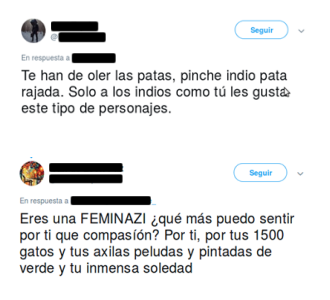
\includegraphics[width=0.5\textwidth]{img/tweets_ofensivos.png}
	\caption{Ejemplos de mensajes ofensivos en Twitter}
	\label{fig:tweets_ofensivos}
\end{figure}

\clearpage
\subsubsection{Alcance y Limitaciones}
\paragraph{}
En este trabajo se abarca el diseño e implementación y de un programa para detectar lenguaje ofensivo dentro de la red social Twitter
El conjunto de datos utilizado proviene de foros de discusión sobre comentarios publicados en la red social Twiter (tweets). Estos 'tweets' fueron recuperados de diferentes publicaciones y se fueron clasificando en tweets 'ofensivos' y 'no ofensivos'

Para el desarrollo de la solución se trabajará con un descriptor llamado 'Bolsa de palabras' el cual realizará el trabajo de convertir determinadas palabras en vectores para que se puedan trabajar; seguidamente usaremos un reductor de dimensiones 'MDS' con la finalidad de reducir las dimensiones de los vectores generados con el descriptor y de esta manera pasar a la manipulacion de los mismos con el uso del algoritmo de KNN donde se tendrá una etapa de aprendizaje con ejemplos reconocidos de forma manual (al cual llamaremos aprendizaje) para despues pasar al modo pruebas con datos nuevos y aleatorios donde el algoritmo KNN realizará la clasificación de las entradas. 

\subsubsection{Descriptor: Bolsa de Palabras}
\paragraph{}
BoVW es actualmente un método popular para el reconocimiento de objetos y escenas en visión por computadoras. A una imagen se le extraen los rasgos locales y pasa a ser considerada como una bolsa de rasgos (bag of features), es decir, ignorando las relaciones espaciales entre ellos. Como desventaja podemos mencionar que este no cuenta con un mecanismo eficiente y efectivo de codificación de la información espacial que existe para los rasgos. Un método basado en el BoVW clásico consiste en las siguientes etapas:

\begin{figure}[h!]
	\centering
	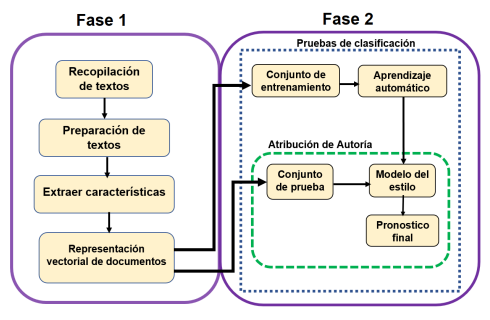
\includegraphics[width=0.7\textwidth]{img/diagrama_bloques.png}
	\caption{Diagramas de bloques de la \textit{Bolsa de Palabras}}
	\label{fig:diagrama_bloques}
\end{figure}

\begin{enumerate}
	\item \textbf{Extracción de rasgos:} Los rasgos locales y sus descriptores correspondientes se extraen de parches locales de la imagen. Los dos descriptores visuales más usados son SIFT (LOWE, 2004) y SURF (VEDALDI and FULKERSON, 2010). Algunos métodos los extraen en ciertos puntos de interés detectados y otros obtienen los rasgos locales densamente, en posiciones regulares de la imagen por ejemplo PHOW (VEDALDI  and  FULKERSON,  2010).
	\item \textbf{Generar un diccionario y mapear los rasgos a palabras visuales:} Un diccionario visual es un método que divide el espacio de descriptores visuales en varias regiones. Los rasgos de una región corresponden a la misma palabra visual. Entonces, una imagen se codifica como un histograma de la frecuencia de ocurrencia de cada palabra visual. Esto se hace asignando a cada vector de rasgos de la imagen su región más cercana, de manera que al terminar el proceso se tenga la cantidad de vectores asignados a cada región y se asigna esa cantidad a la componente correspondiente a esa palabra visual en el histograma.
	\item \textbf{Entrenar y probar:} Varios métodos de aprendizaje por computadora pueden aplicarse para la representación de imágenes usada. SVM es frecuentemente usado como clasificador en modelos BoVW para el reconocimiento de objetos y escenas. Este fue el clasificador escogido para resolver el problema planteado, en conjunto con el kernel aditivo de intersección de histogramas debido a su utilidad y buen desempeño para representaciones basadas en histogramas.
\end{enumerate}

\subsubsection{Reductor de Dimensiones MDS}
\paragraph{}

\textit{Multidimensional scaling} es un método para representar una matriz de disimilaridades en un cierto número de dimensiones. Se puede usar como una técnica de reducción de la dimensionalidad si se calculan las disimilaridades con respecto a la dimensión original y luego se representan en un espacio de dimensión menor.

La idea de MDS es que las distancias euclídeas en el espacio de llegada sean lo más cercanas posibles a las disimilaridades en el espacio original. Si tenemos observaciones $x_1, x_2..., x_N$ y una función de disimilaridad \textit{d}, la función de coste a optimizar en MDS podría ser:

\[C=\sum_{i \neq j}^{}(d(x_i,x_j)-||z_i-z_j||)^2\]

donde $z_i$ y $z_j$ son los representantes en el espacio de llegada de $x_i$ y $x_j$ respectivamente.
Esta función puede optimizarse mediante descenso del gradiente

Sin embargo, si nuestras disimilaridades son distancias euclídeas existe una solución analítica. Si nuestras observaciones originales se representan por la matriz X sabemos que la matriz de Gram se define como $B = XX^T$. Podemos obtener la matriz de Gram mediante nuestra matriz de distancias al cuadrado D.

\[B=\frac{-1}{2} * C_n * D * C_n\]

Donde $C_n = I_n - \frac{1}{n} 11^T$ sirve para centrar la matriz de distancias. Por tanto si descomponemos la matriz de Gram podremos recuperar la matriz X y con ella las coordenadas en el espacio de llegada. En este caso (usando distancias euclídeas) el resultado será equivalente al obtenido mediante PCA.

\subsubsection{KNN}
K-Nearest Neighbors es uno de los algoritmos de clasificación más básicos pero esenciales en Machine Learning. Pertenece al dominio de aprendizaje supervisado y encuentra una intensa aplicación en el reconocimiento de patrones, minería de datos y detección de intrusos.
Es ampliamente disponible en escenarios de la vida real ya que no es paramétrico, lo que significa que no hace suposiciones subyacentes sobre la distribución de datos (a diferencia de otros algoritmos como GMM, que asume una distribución gaussiana de los datos dados) .
Nos dan unos datos previos (también llamados datos de entrenamiento), que clasifican las coordenadas en grupos identificados por un atributo.
Como ejemplo, considere la figura \ref{fig:knn_01} que muestra una tabla de puntos de datos que contienen dos características:

\begin{figure}[h!]
	\centering
	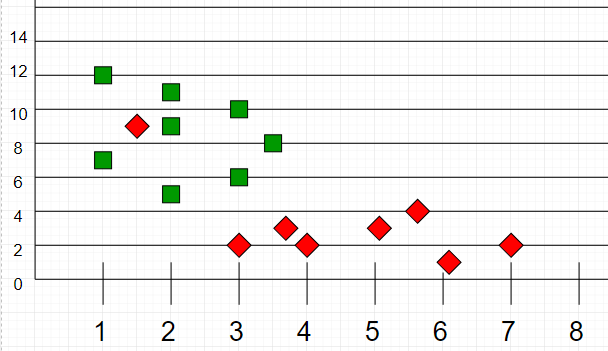
\includegraphics[width=0.5\textwidth]{img/knn_01.png}
	\caption{Datos de entrenamiento en KNN}
	\label{fig:knn_01}
\end{figure}

Ahora, dado otro conjunto de puntos de datos (también llamados datos de prueba), asigne estos puntos a un grupo analizando el conjunto de entrenamiento. Tenga en cuenta que los puntos no clasificados están marcados como 'Blanco', de acuerdo la la figura \ref{fig:knn_02}

\begin{figure}[h!]
	\centering
	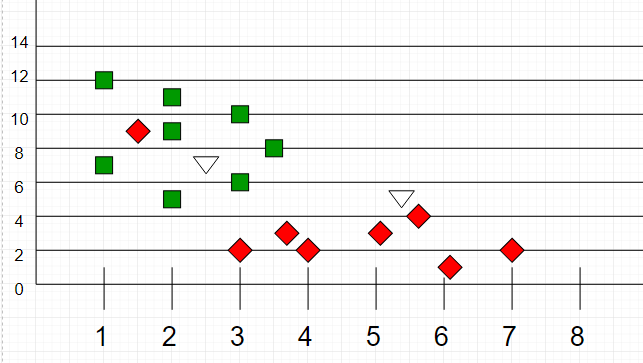
\includegraphics[width=0.5\textwidth]{img/knn_02.png}
	\caption{Datos de prueba en KNN}
	\label{fig:knn_02}
\end{figure}

\paragraph{Intuición}
Si trazamos estos puntos en un gráfico, podemos ubicar algunos grupos o grupos. Ahora, dado un punto sin clasificar, podemos asignarlo a un grupo observando a qué grupo pertenecen sus vecinos más cercanos. Esto significa que un punto cercano a un grupo de puntos clasificados como 'Rojo' tiene una mayor probabilidad de ser clasificado como "Rojo".
Intuitivamente, podemos ver que el primer punto (2.5, 7) debe clasificarse como 'Verde' y el segundo punto (5.5, 4.5) debe clasificarse como 'Rojo'.

\paragraph{Algoritmo}
Sea m el número de muestras de datos de entrenamiento. Sea p un punto desconocido.
\begin{enumerate}
	\item Almacene las muestras de entrenamiento en una matriz de puntos de datos arr[ ]. Esto significa que cada elemento de esta matriz representa una tupla (x, y).
	\item Haz el conjunto S de las K distancias más pequeñas obtenidas. Cada una de estas distancias corresponde a un punto de datos ya clasificado.
	\item Devuelve la etiqueta mayoritaria entre S.
\end{enumerate}

\paragraph{}
K se puede mantener como un número impar para que podamos calcular una clara mayoría en el caso de que solo sean posibles dos grupos (por ejemplo, rojo/azul). Con el aumento de K, obtenemos límites más suaves y definidos a través de diferentes clasificaciones. Además, la precisión del clasificador anterior aumenta a medida que aumentamos la cantidad de puntos de datos en el conjunto de entrenamiento.

\clearpage
\section{Programa}

\subsection{Descripcion del Programa}
\paragraph{}
Para el desarrollo de la solución se trabajará con un descriptor llamado 'Bolsa de palabras' el cual realizará el trabajo de convertir determinadas palabras en vectores para que se puedan trabajar; seguidamente usaremos un reductor de dimensiones 'MDS' con la finalidad de reducir las dimensiones de los vectores generados con el descriptor y de esta manera pasar a la manipulacion de los mismos con el uso del algoritmo de KNN donde se tendrá una etapa de aprendizaje con ejemplos reconocidos de forma manual (al cual llamaremos aprendizaje) para despues pasar al modo pruebas con datos nuevos y aleatorios donde el algoritmo KNN realizará la clasificación de las entradas.

\clearpage
\subsection{Partes del Programa}

\subsubsection{Algoritmo KNN}
En la figura \ref{fig:knn_03} se muestra el código desarrollado para la ejecución del algoritmo \textit{KNN}

\begin{figure}[h!]
	\centering
	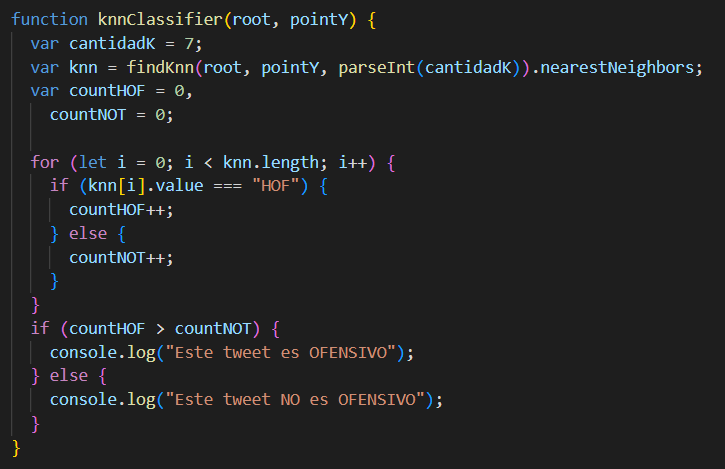
\includegraphics[width=0.7\textwidth]{img/knn_03.png}
	\caption{Código en\textit{javascript}} para el desarrollo del algoritmo \textit{KNN}
	\label{fig:knn_03}
\end{figure}

\clearpage
\subsubsection{Algoritmo Descriptor "Bolsa de Palabras"}
En la figura \ref{fig:bolsa_palabras} se muestra parte del código del descriptor denominado 'bolsa de palabras'.

\begin{figure}[h!]
	\centering
	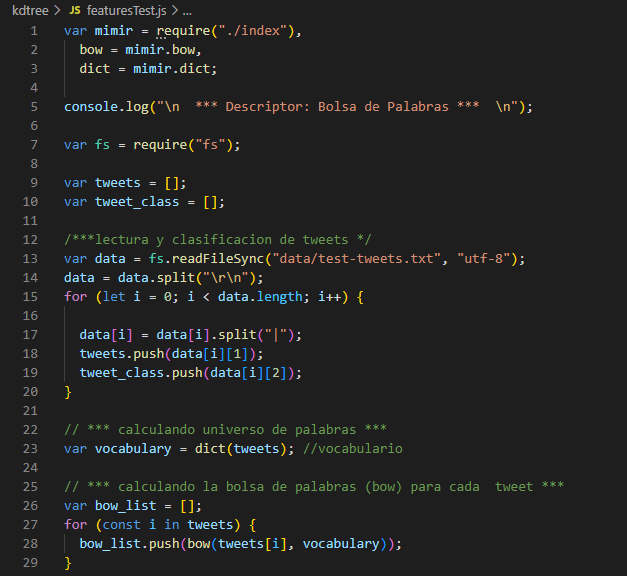
\includegraphics[width=0.7\textwidth]{img/bolsa_palabras.png}
	\caption{Código del algoritmo \textit{bolsa de palabras}}
	\label{fig:bolsa_palabras}
\end{figure}

\clearpage
\subsubsection{Algoritmo Reductor de Dimensiones "MDS"}
En la figura \ref{fig:mds} se muestra el codigo del algoritmo MDS\textit{closest\_point\_force\_brute}.

\begin{figure}[h!]
	\centering
	\includegraphics[width=0.7\textwidth]{img/mds.png}
	\caption{Código del algoritmo \textit{MDS}}
	\label{fig:mds}
\end{figure}

\clearpage
\subsubsection{Ejecución del Programa}

\begin{figure}[h!]
	\centering
	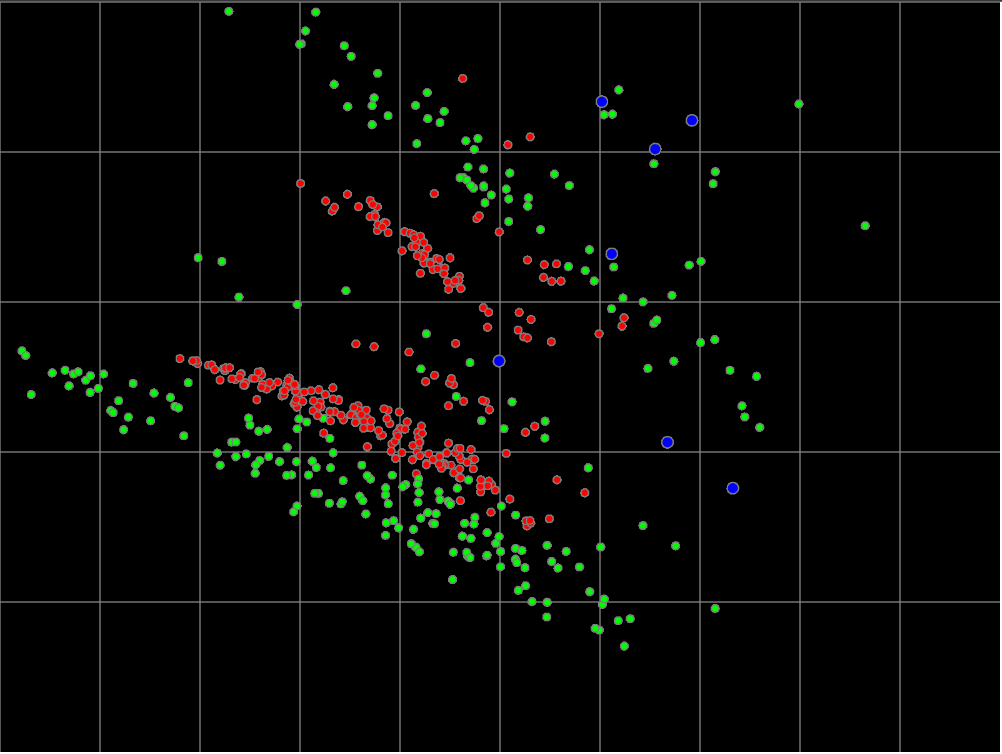
\includegraphics[width=0.6\textwidth]{img/knn_05.png}
	\caption{Representacion grafica de la clasificación de tweets ofensivos (puntos rojos) y no ofensivos (puntos verdes) por \textit{KNN}}
	\label{fig:knn_05}
\end{figure}

\begin{figure}[h!]
	\centering
	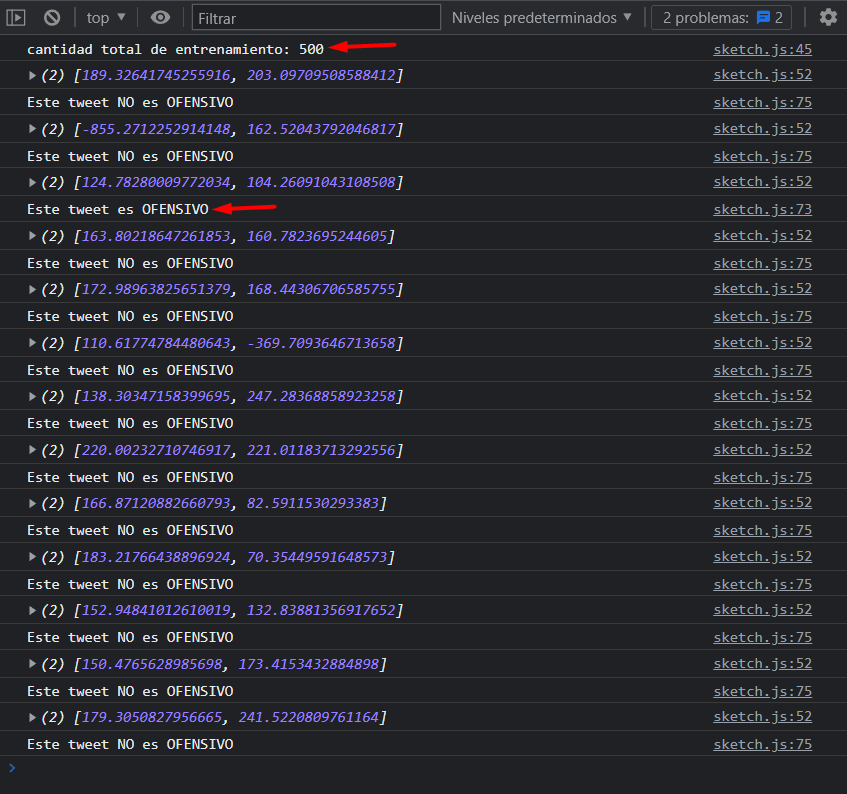
\includegraphics[width=0.6\textwidth]{img/knn_06.png}
	\caption{Clasificación de tweets de prueba (representados por puntos azules) \textit{KNN}}
	\label{fig:knn_06}
\end{figure}

\clearpage
\section{Conclusiones}
\begin{itemize}
	\item Durante la pruebas del KNN Classifier se pudo observar que hay casos en los que el clasificador falla, sobre todo en las zonas en las que se solapan los tweets ofensivos y no ofensivos.
	\item Los algoritmos de clasificación no son 100% precisos, tienen un grado de certeza que varía dependiendo de la data utilizada durante el entrenamiento, de los algoritmos de reducción de dimensiones aplicados, y de las características a tomar en cuenta
	\item Usando la reducción de dimensiones MDS se logró condicionar la matriz obtenida de la Bolsa de Palabras, lo cual permitió utilizar el algoritmo KDtree y KNN para 2 dimensiones
	
\end{itemize}

\section{Referencias}
\begin{enumerate}
	\item Amalia Duch, Vladimir Estivill-Castro, Conrado Martínez, “Randomized K-Dimensional Binary Seach Trees”, M-RR/LSI-98-48-R, Universitat Politècnica de Catalunya, Barcelona, 1998.
	\item C. Martínez y S. Roura, “Randomized binary search trees”, Journal of the ACM, Marzo 1998, Volumen 45, núm. 2, 288$–$323.
	\item W. Cunto, G. Lau, y Ph. Flajolet, “Analysis of kd-trees: kd-trees improved by local reorganizations”, In F. Dehne, J. R. Sack y N. Santoro editors, Work, Algorithms and Data Structures, 1989, Volumen 382, 24$–$38.
	\item Andrew W. Moore, “An Introductory tutorial on kd-trees”, Carnegie Mellon University, awm@cs.cmu.edu, 1992. http://www.autonlab.org.
	\item Luc Devroye, Nicholas Broutin, Ketan Dalal y Erin McLeish, “The kdtreap”, Personal Communication.
	\item \href{https://www.redseguridad.com/revistas/red/095/58/index.html}{Redseguridad}
	\item \href{https://www.ccn-cert.cni.es/informes/informes-ccn-cert-publicos/5377-ccn-cert-ia-13-20-ciberamenazas-y-tendencias-edicion-2020/file.html}{ccn-cert}
	\item \href{https://www.geeksforgeeks.org/}{Geeksforgeeks}
\end{enumerate}

\end{document}
